% SPDX-License-Identifier: CC-BY-4.0
%
% Copyright (c) 2023 Nelson Vieira
%
% @author Nelson Vieira <nelson0.vieira@gmail.com>
% @license CC-BY-4.0 <https://creativecommons.org/licenses/by/4.0/legalcode.txt>
\documentclass[xcolor={svgnames},compress,aspectratio=169]{beamer}
\usetheme{Berlin}
\usecolortheme{dolphin}

\setbeamercolor*{structure}{bg=Azure,fg=MidnightBlue!50!black}

\setbeamercolor*{palette primary}{use=structure,fg=structure.bg,bg=structure.fg}
\setbeamercolor*{palette secondary}{use=structure,fg=structure.fg,bg=structure.bg}
\setbeamercolor*{palette tertiary}{use=structure,fg=structure.fg,bg=GhostWhite}
\setbeamercolor*{palette quaternary}{fg=white,bg=black}

\setbeamercolor{section in head/foot}{parent=palette primary} % Outer section of header/footer
\setbeamercolor{subsection in head/foot}{parent=palette secondary} % Inner section of header/footer

\setbeamercolor{titlelike}{parent=palette tertiary} % Main titles
\setbeamercolor{frametitle}{parent=palette tertiary,bg=GhostWhite!50}

\setbeamercolor{section in toc}{fg=darkgray,bg=Azure} % Table of contents sections
\setbeamercolor{subsection in toc}{fg=darkgray,bg=Azure} % Table of contents subsections
% \setbeamercolor{alerted text}{use=structure,fg=structure.fg!50!black!80!black}

% \setbeamertemplate{navigation symbols}{} % Hides navigation buttons at the bottom
% \setbeamertemplate{headline}{} % Hides navigation bar at the top

\setbeamercovered{transparent}

\setbeamertemplate{caption}[numbered]

% \usepackage{pgfpages}
% \pgfpagesuselayout{4 on 1}[a4paper,border shrink=5mm]

\usepackage[utf8]{inputenc}
\usepackage{adjustbox}
\usepackage{xcolor,colortbl}
\usepackage[all]{xy}
\usepackage{tikz}
\usetikzlibrary{mindmap,backgrounds}
\usepackage{graphicx}
\usepackage{multicol}
% Advanced table functions
\usepackage{tabularx,ragged2e}
\usepackage{booktabs}
% Listings extension
\usepackage{listings}
\usepackage{svg}
\setsvg{inkscape = "C:/Program Files/Inkscape/bin/inkscape.exe" -z -D}
\svgsetup{inkscapepath=svgsubdir}
\def\myversion{0.1}

\title[Privacy in the Internet of Things: Fostering User Empowerment through Digital Literacy]{Master's Dissertation \\ {\normalsize Privacy in the Internet of Things: Fostering User Empowerment through Digital Literacy}}
% \subtitle{Empowering Users' Privacy Rights in the Internet of Things}
\author{\href{mailto:2080511@student.uma.pt}{Nelson Vieira}
\\ \and \textcolor{gray}{Orientation} \href{mailto:mary.barreto@staff.uma.pt}{Mary Barreto}
}
\institute[\href{https://www.uma.pt/}{University of Madeira}]{University of Madeira\\Faculty of Exact Sciences and Engineering}
\date{{\scriptsize Last Update: \today}}

\setbeameroption{hide notes}

\makeatletter
    \newenvironment{withoutheadline}{
        \setbeamertemplate{headline}[default]
        \def\beamer@entrycode{\vspace*{-\headheight}}
    }{}
\makeatother

\begin{document}

\begin{withoutheadline}
    \begin{frame}
        \centering
\includegraphics[width=90pt]{../thesis/assets/images/uma_logo.png}
        \maketitle
    \end{frame}
\end{withoutheadline}

\begin{frame}{Table of Contents}
    % Use hideallsubsections for longer presentations
    % \tableofcontents[hideallsubsections]
    \begin{multicols}{2}
        \tableofcontents
    \end{multicols}
\end{frame}

\section{Introduction}

\begin{frame}{Introduction}
    % Internet of Things (IoT) devices are everywhere. These devices
    % create new ways of collecting and process personal data from users and
    % non-users. Most end users are not even aware or have little control over
    % the information that is being collected by these systems.

    This work takes an holistic approach to this problem by doing:
    \begin{itemize}
        \item<1-> Systematic literature review;
        \item<2-> A survey;
        \item<3-> A mobile application.
    \end{itemize}
\end{frame}

\begin{frame}{Privacy}
    \begin{multicols}{2}
        \centering
        \vspace*{\fill}
        What is privacy?
        % \begin{figure}
        %     \centering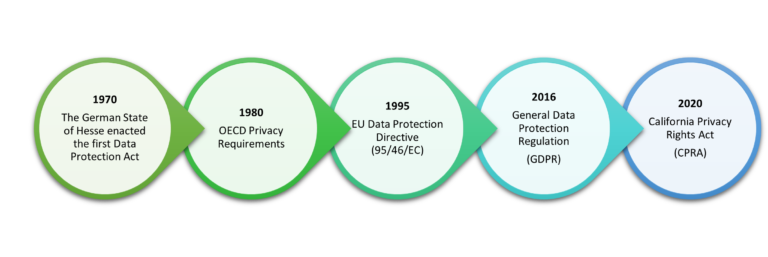
\includegraphics[width=200pt]{assets/images/privacy_history.png}
        %     \caption{Privacy history}
        % \end{figure}
        \vspace*{\fill}

        \columnbreak
        % \onslide*<2>
        \centering
        \vspace*{\fill}
        Privacy $\ne$ Security
        \vspace*{\fill}
    \end{multicols}
\end{frame}

\begin{frame}{Internet of Things}
\end{frame}

\section{State of the Art}

\begin{frame}{State of the Art}
\end{frame}

\subsection{Literature Approaches}

\begin{frame}{Literature Approaches}
\end{frame}

\section{Methodology}

% \subsection{Survey}

% \begin{frame}[shrink]{Survey}
    % \begin{multicols}{2}
    %     92 Questions
    %     \begin{itemize}
    %         \item General knowledge and attitudes towards privacy
    %         \item Disposition for sharing personal information
    %         \item Privacy concerns
    %         \item Current online habits and practices
    %         \item Profile identification
    %         \item Knowledge and habits regarding the Internet of Things
    %         \item Demographic data
    %     \end{itemize}

    %     \columnbreak
    %     \begin{figure}
    %         \centering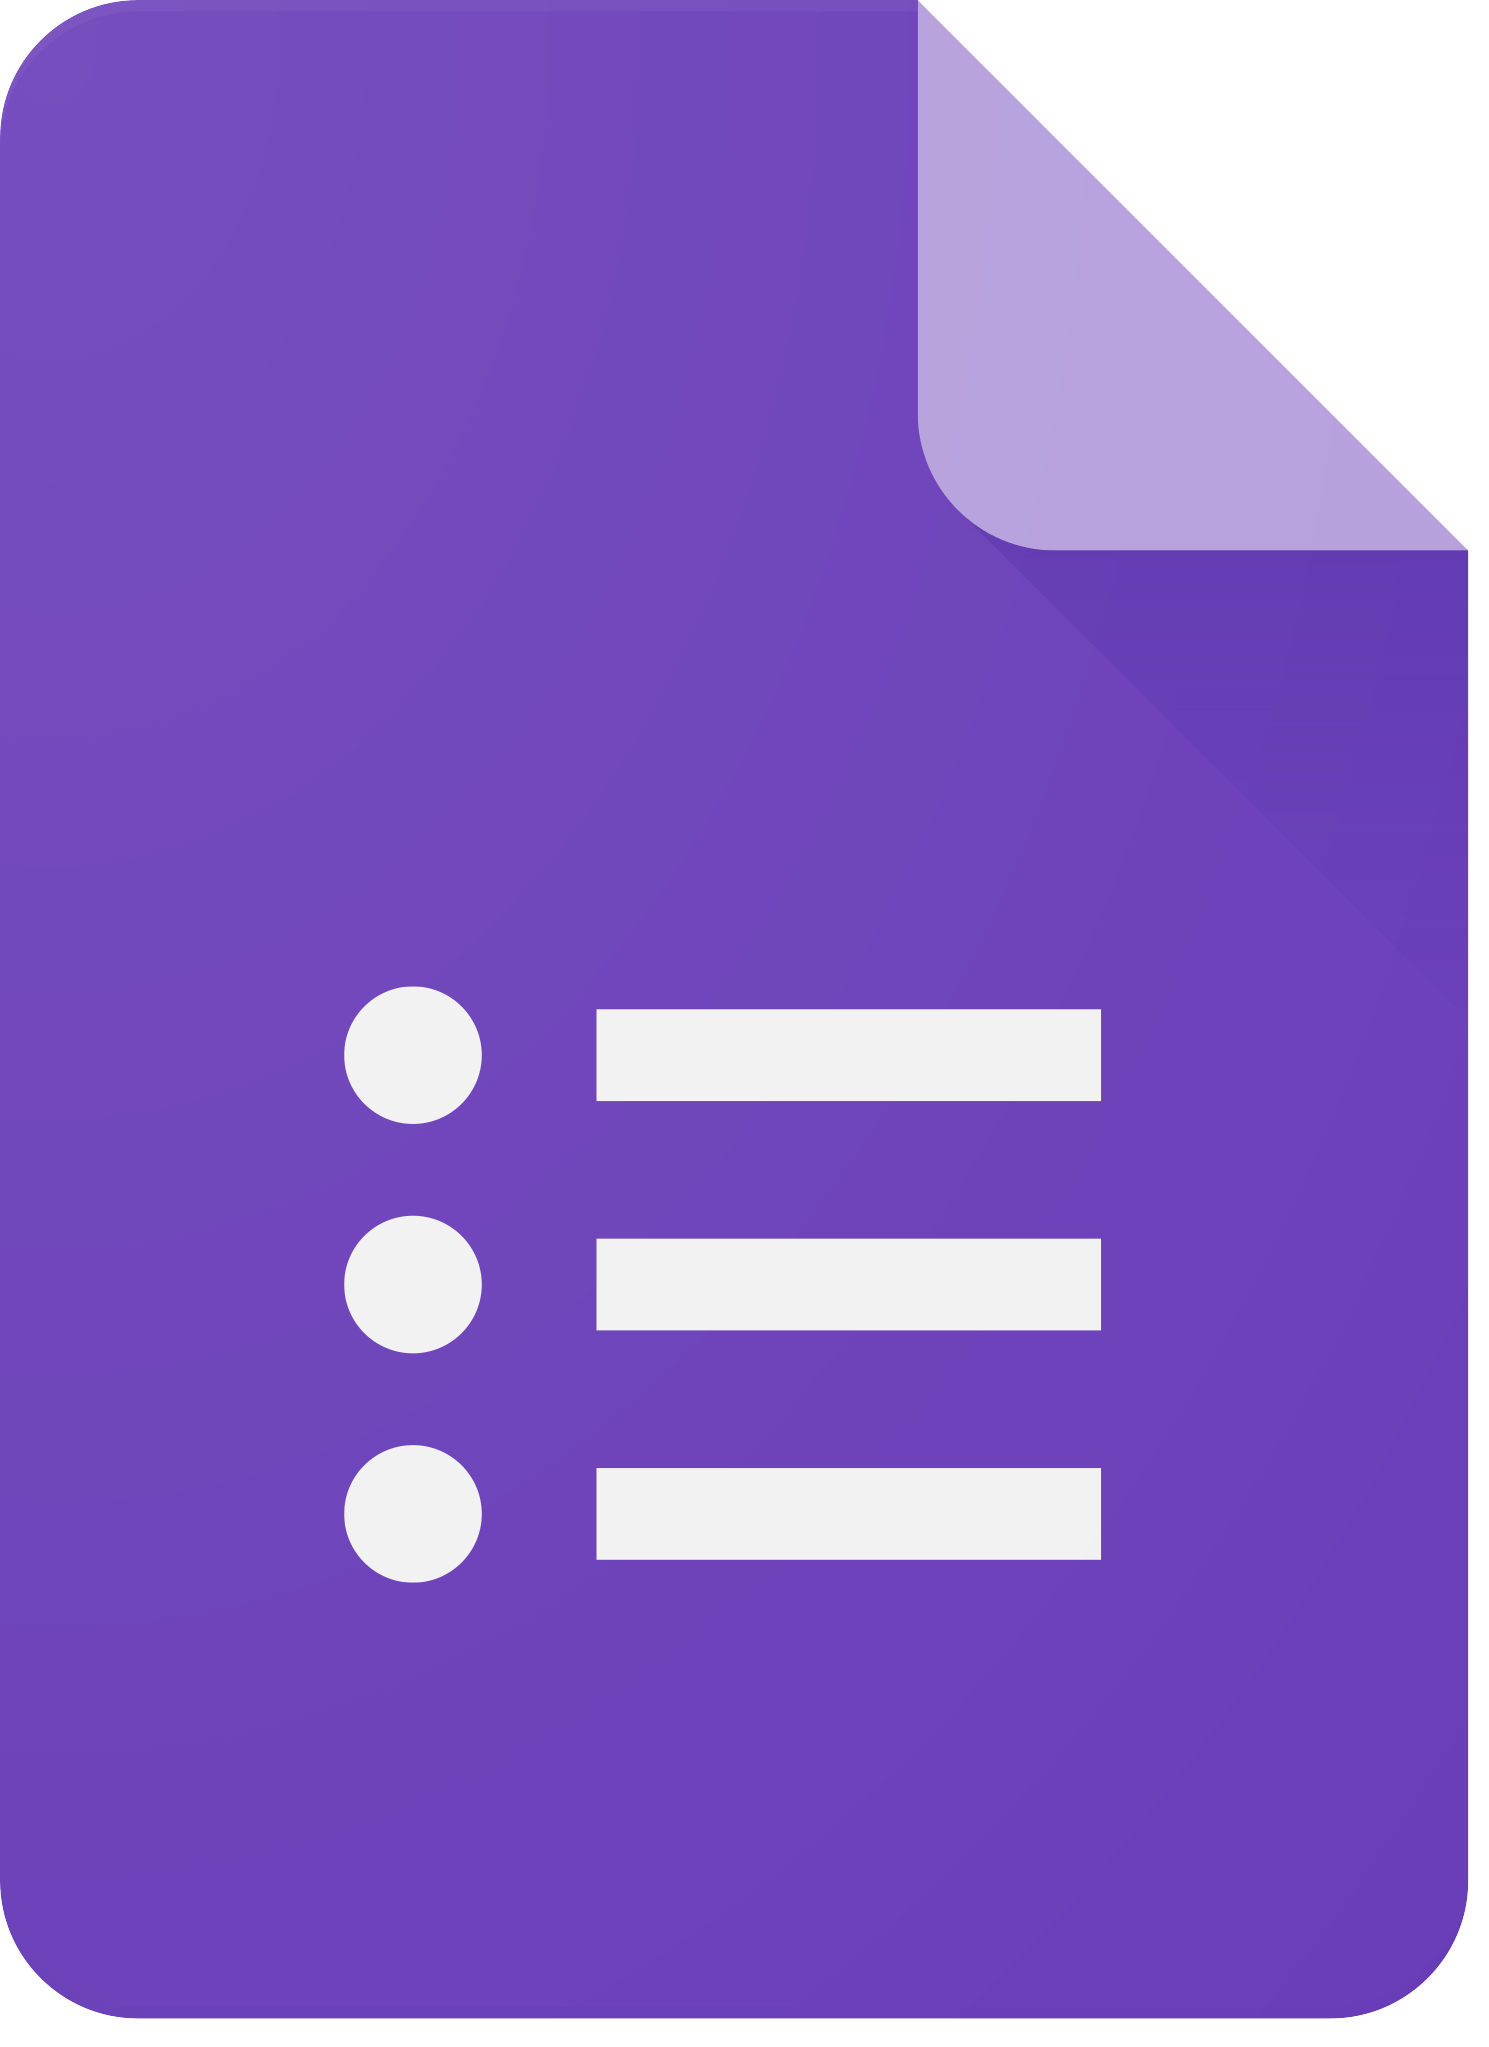
\includegraphics[width=45pt]{assets/images/forms.png}
    %         \caption{Google Forms}
    %     \end{figure}
    % \end{multicols}
% \end{frame}

\subsection{Application}

\begin{frame}{Application}
    % \begin{multicols}{2}
    %     Will be composed of the following things:
    %     \begin{itemize}
    %         \item Show the geolocation of the IoT devices;
    %         \item What type of device it is;
    %         \item What type of data is being collect by the device;
    %         \item Insert IoT devices and associated information about them.
    %     \end{itemize}

    %     \columnbreak
    %     \begin{figure}
    %         \centering
\includegraphics[width=120pt]{assets/images/flutter.png}
    %         \caption{Flutter framework}
    %     \end{figure}
    %     \begin{figure}
    %         \centering
    %         \includesvg{assets/images/firebase}
    %         \caption{Firebase cloud backend}
    %     \end{figure}
    % \end{multicols}
\end{frame}

\section{Conclusion and Future Work}

\subsection{Future Work}

\begin{frame}{Future Work}
\end{frame}

\subsection{Conclusion}

\begin{frame}{Conclusion}
    % This project aims to do an exploratory analysis of privacy in
    % IoT systems. It proposes a survey to better understand user's
    % knowledge on this subject and an application that aims to
    % create more users awareness and better inform about their
    % environment, as well as the IoT devices that inhabit it and
    % how they can respond accordingly.
\end{frame}

\begin{frame}{Questions and Comments}
    Thank you for your attention. Any questions?
\end{frame}

\subsection{References}

\begin{frame}[allowframebreaks]{References}
    \bibliographystyle{IEEEtran}
    \bibliography{assets/references}
\end{frame}

\end{document}
